\chapter{معرفی یادگیری ماشین}
\section{مقدمه}
\subsection{جایگاه یادگیری تقویتی در یادگیری ماشین}
بسیاری از صاحب نظران یادگیری ماشین را 
\begin{figure}
	\centering
	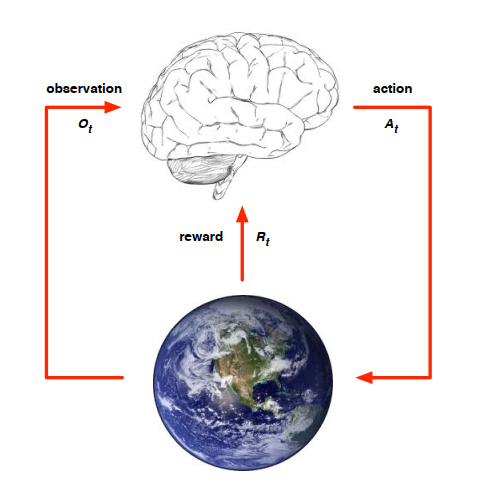
\includegraphics[width=0.7\linewidth]{Figures/RL/Enviroment-brain-as-agent}
	\caption{}
	\label{fig:enviroment-brain-as-agent}
\end{figure}
\begin{figure}
	\centering
	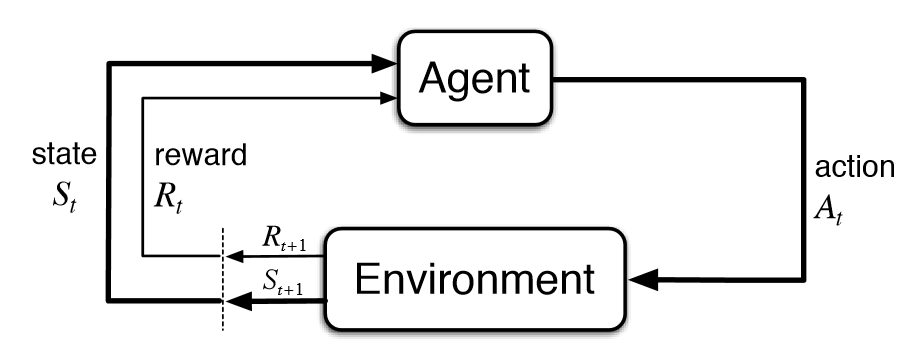
\includegraphics[width=0.7\linewidth]{Figures/RL/Markov-vhain-SARSA}
	\caption{}
	\label{fig:markov-vhain-sarsa}
\end{figure}
\begin{figure}
	\centering
	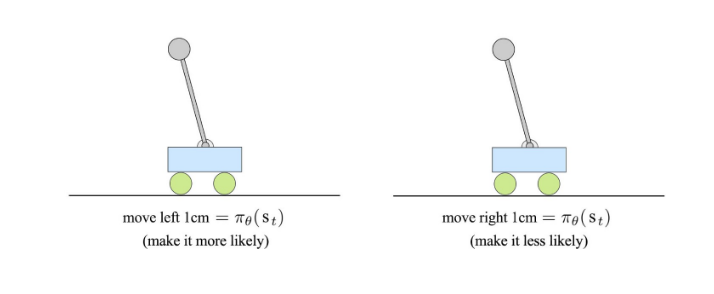
\includegraphics[width=0.7\linewidth]{Figures/RL/RL-cartpole}
	\caption{}
	\label{fig:rl-cartpole}
\end{figure}
\begin{figure}
	\centering
	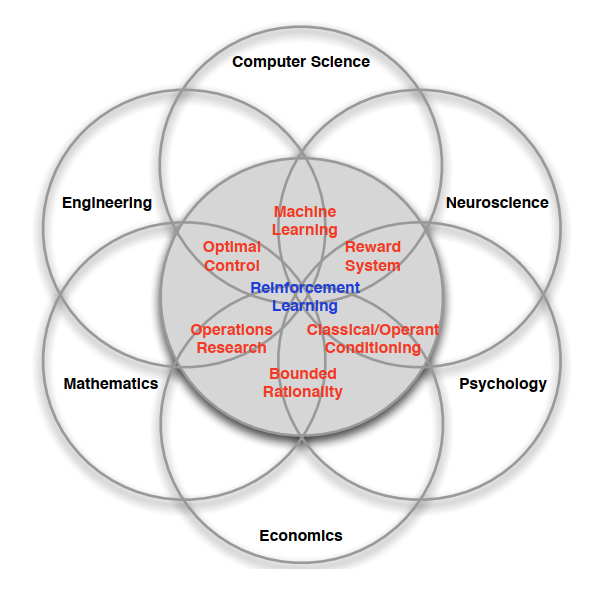
\includegraphics[width=0.7\linewidth]{Figures/RL/RL-chart}
	\caption{}
	\label{fig:rl-chart}
\end{figure}
